% Indicate the main file. Must go at the beginning of the file.
% !TEX root = ../main.tex

%%%%%%%%%%%%%%%%%%%%%%%%%%%%%%%%%%%%%%%%%%%%%%%%%%%%%%%%%%%%%%%%%%%%%%%%%%%%%%%%
% SECTION 1
%%%%%%%%%%%%%%%%%%%%%%%%%%%%%%%%%%%%%%%%%%%%%%%%%%%%%%%%%%%%%%%%%%%%%%%%%%%%%%%%

\section{Introduction}
\label{section1}
\kant[1]

\begin{itemize}
\item None
\item Some
\item Every
\end{itemize}

\kant[2]

\begin{figure}[h!]
    \centering
%    \captionsetup{width=.7\linewidth}
    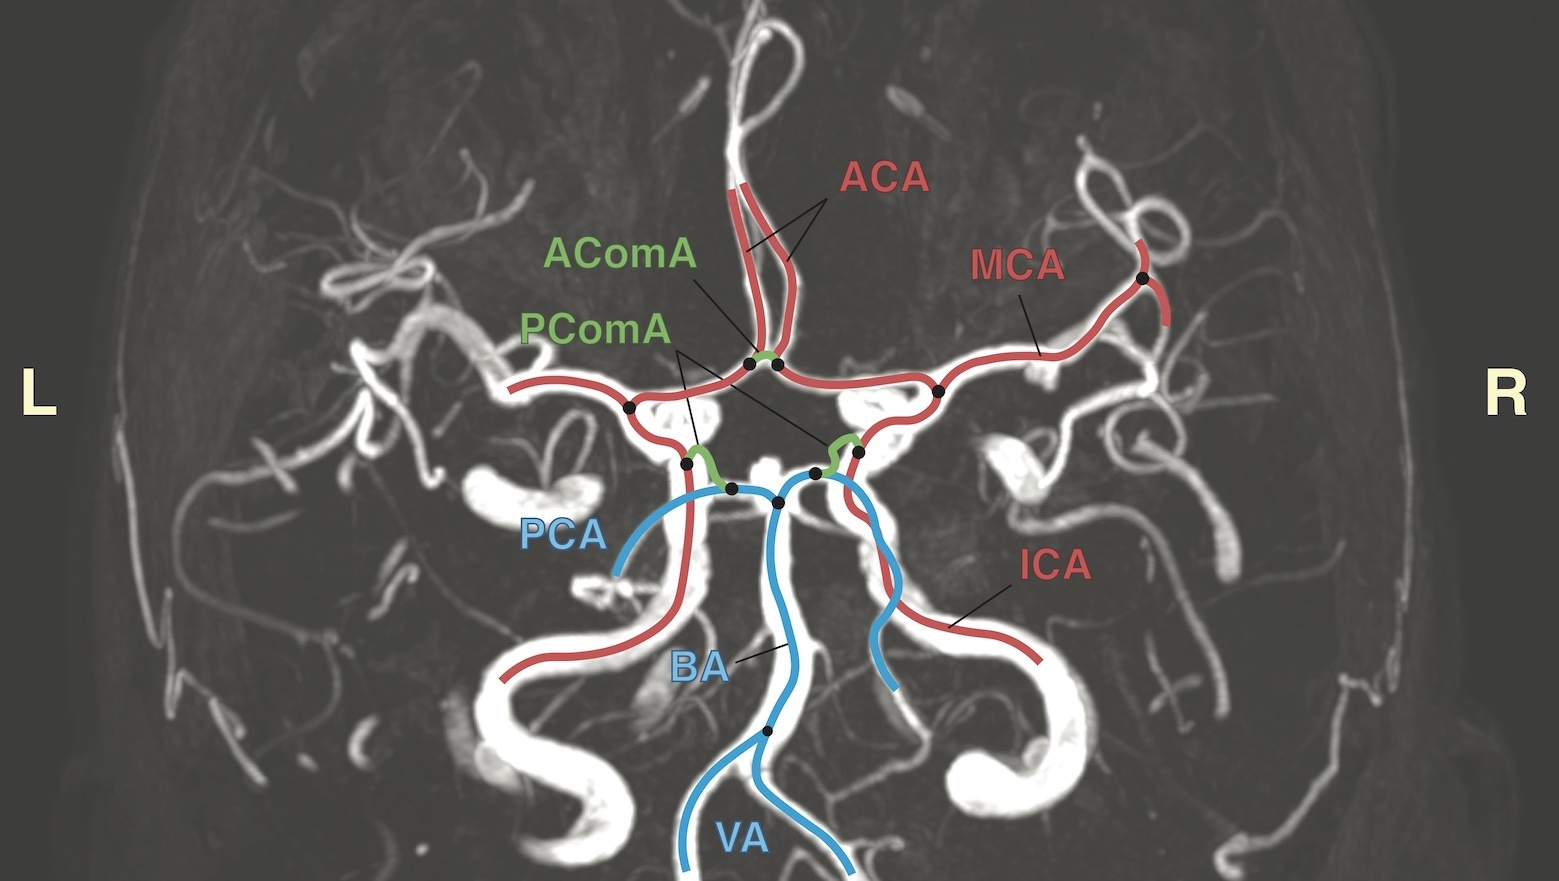
\includegraphics[width=0.85\textwidth]{figures/cow_contrast_lowres.jpg}
    \caption{Some random image without meaning.}
    \label{fig:1:illustration}
\end{figure}
\newpage

\kant[1-2]

\begin{figure}[ht]
  \centering
  \begin{subfigure}[b]{0.45\textwidth}
    \centering
    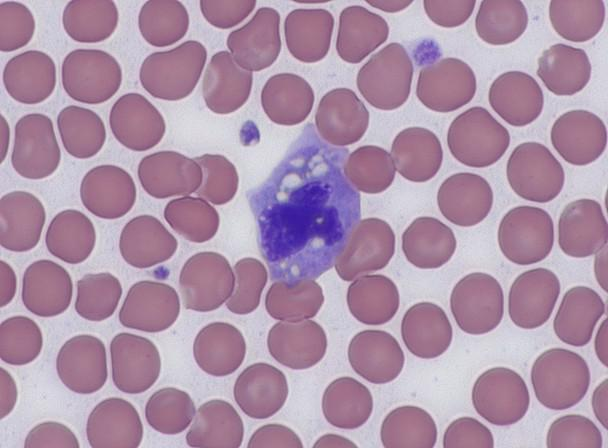
\includegraphics[width=\textwidth]{figures/mono.jpg}
    \label{fig:1:mono}
    \vspace{-0.5cm}
    \caption{Some cell without meaning.}
  \end{subfigure}
  %\hspace{0.5cm}
  \hfill
  \begin{subfigure}[b]{0.45\textwidth}
    \centering
    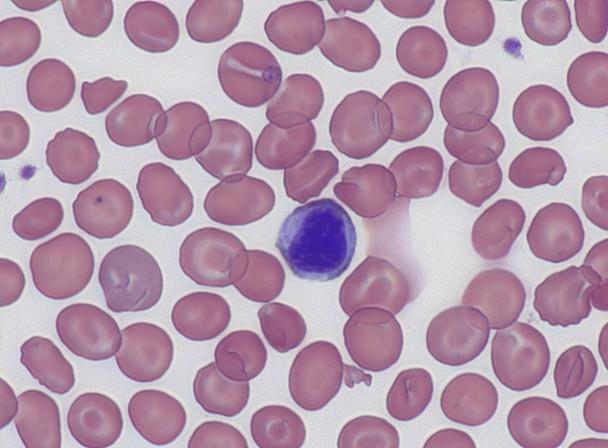
\includegraphics[width=\textwidth]{figures/lymph.jpg}
    \label{fig:1:lymph}
    \vspace{-0.5cm}
    \caption{Some other cell without meaning.}
  \end{subfigure}
  \caption{Here, we present some biology without (you guessed it) deeper meaning. Look at the colorful dot in the middle of the image.}
  \label{fig:samples_full_size}
\end{figure}

